\documentclass[12pt]{amsart}
\usepackage{../marktext} 
%% Remove draft for real article, put twocolumn for two columns
\usepackage{../svmacro}
\usepackage[utf8]{inputenc}
\usepackage{lineno}
%\usepackage{authblk}
\usepackage[style=alphabetic, backend=biber]{biblatex}
\usepackage{enumitem}

%% commentary bubble
\newcommand{\SV}[2][]{\sidenote[colback=green!10]{\textbf{SV\xspace #1:} #2}}

%% Title 
\title{ MATH 170: Homework 2 }
%\author[1]{Co-author}
\author{Due: September 17, 2021}
%\affil[1]{Institute}
\date{}

\begin{document}

\maketitle


\noindent{\bf Graded for accuracy:}
3.
\\
\noindent{\bf Graded for completion:}
1, 2.
\\
\noindent{\bf Instructions:}
Problems that are graded for accuracy must be correct to get points.
Problems that are graded for completion must show some trying effort.

\centerline

\hrule

\centerline

\begin{enumerate}[label=\arabic*.,itemsep=10pt, leftmargin=*]

\item  Are these numbers divisible by 2, 3, 5? To get points, use the criteria of divisibility that we covered in class. Optional: check your answers with a calculator.
    \begin{enumerate}[label=\alph*.,itemsep=5pt, leftmargin=*]
    \item 12345;
    \item 10101010.
    \end{enumerate}

\item  
    \begin{enumerate}[label=\alph*.,itemsep=5pt, leftmargin=*]
    \item Let $a, b \in \mathbb Z$. Prove that $\gcd(a,b) = \gcd(a,-b)$.
    \item Compute $\gcd(12,-30)$ using Euclid's algorithm.
    \item Compute $\gcd(12\,345,11\,100)$ using Euclid's algorithm.
    \item Optional: check your answers on \url{https://www.wolframalpha.com/}.
    \\ 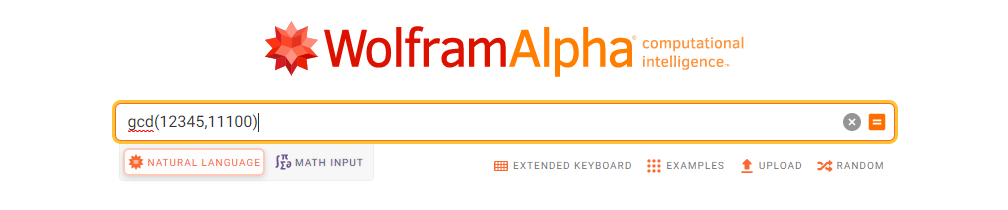
\includegraphics[width=0.9\textwidth]{wolframalpha.png}
    \end{enumerate}

\item
    \begin{enumerate}[label=\alph*.,itemsep=5pt, leftmargin=*]
    \item Divide the following numbers by 10 with remainder: 1234, 2021. That is, write them in the form $10\cdot q + r$, where $0 \leq r < 10$. Compute $1234 + 2021$ and divide the result by 10 with remainder. Observe that the remainder you get is the sum of the first two remainders.
    \item Compute the remainder of $1236$ and $2027$ when dividing by 10, then compute the remainder of their sum. Why is it no longer just the sum of remainders?
    \item Rephrase the following rule in your own words: If you divide $a_1, a_2 \in \mathbb Z$ by $b>0$ with remainder, write the remainder of $a_1$ as $r_1$ and the remainder of $a_2$ as $r_2$. Then the remainder of $a_1 + a_2$ is $r_1 + r_2$ or $r_1 + r_2 - b$.
    
    \item[*]
    Bonus: prove c.
    \end{enumerate}



\end{enumerate}



\end{document}
